\documentclass[./main.tex]{subfiles}

\begin{document}

Since the operation is creating new internal SCM repository at internal GitLab, the whole operation might take several seconds to finish, forcing us to make the operation asynchronous.

The endpoint handler creates the task for this operation. Task logic is done by underlying service, which parses all the necessary information both from the request and from a configuration. For instance, read-only and read-write URLs are composed by completing project path (parsed from request's \textit{project} field) into the read-only and read-write templates\footnote{\url{https://github.com/project-ncl/reqour/blob/akridl-thesis/core/src/main/resources/application.yaml##L14-L15}}.

Once all the required project-related information are acquired, we create the project by GitLab API service, which sends the creation request with all the details. Lastly, the task specifies where and what to send in the callback.

The created task is propagated into asynchronous task executor, which will start the execution on another thread.

Finally, the endpoint handler returns 202 Accepted to inform a client that an operation is being executed.

The design described above is visualized using Figure \ref{fig:internal-scm-design}.

\begin{figure}
  \begin{center}
    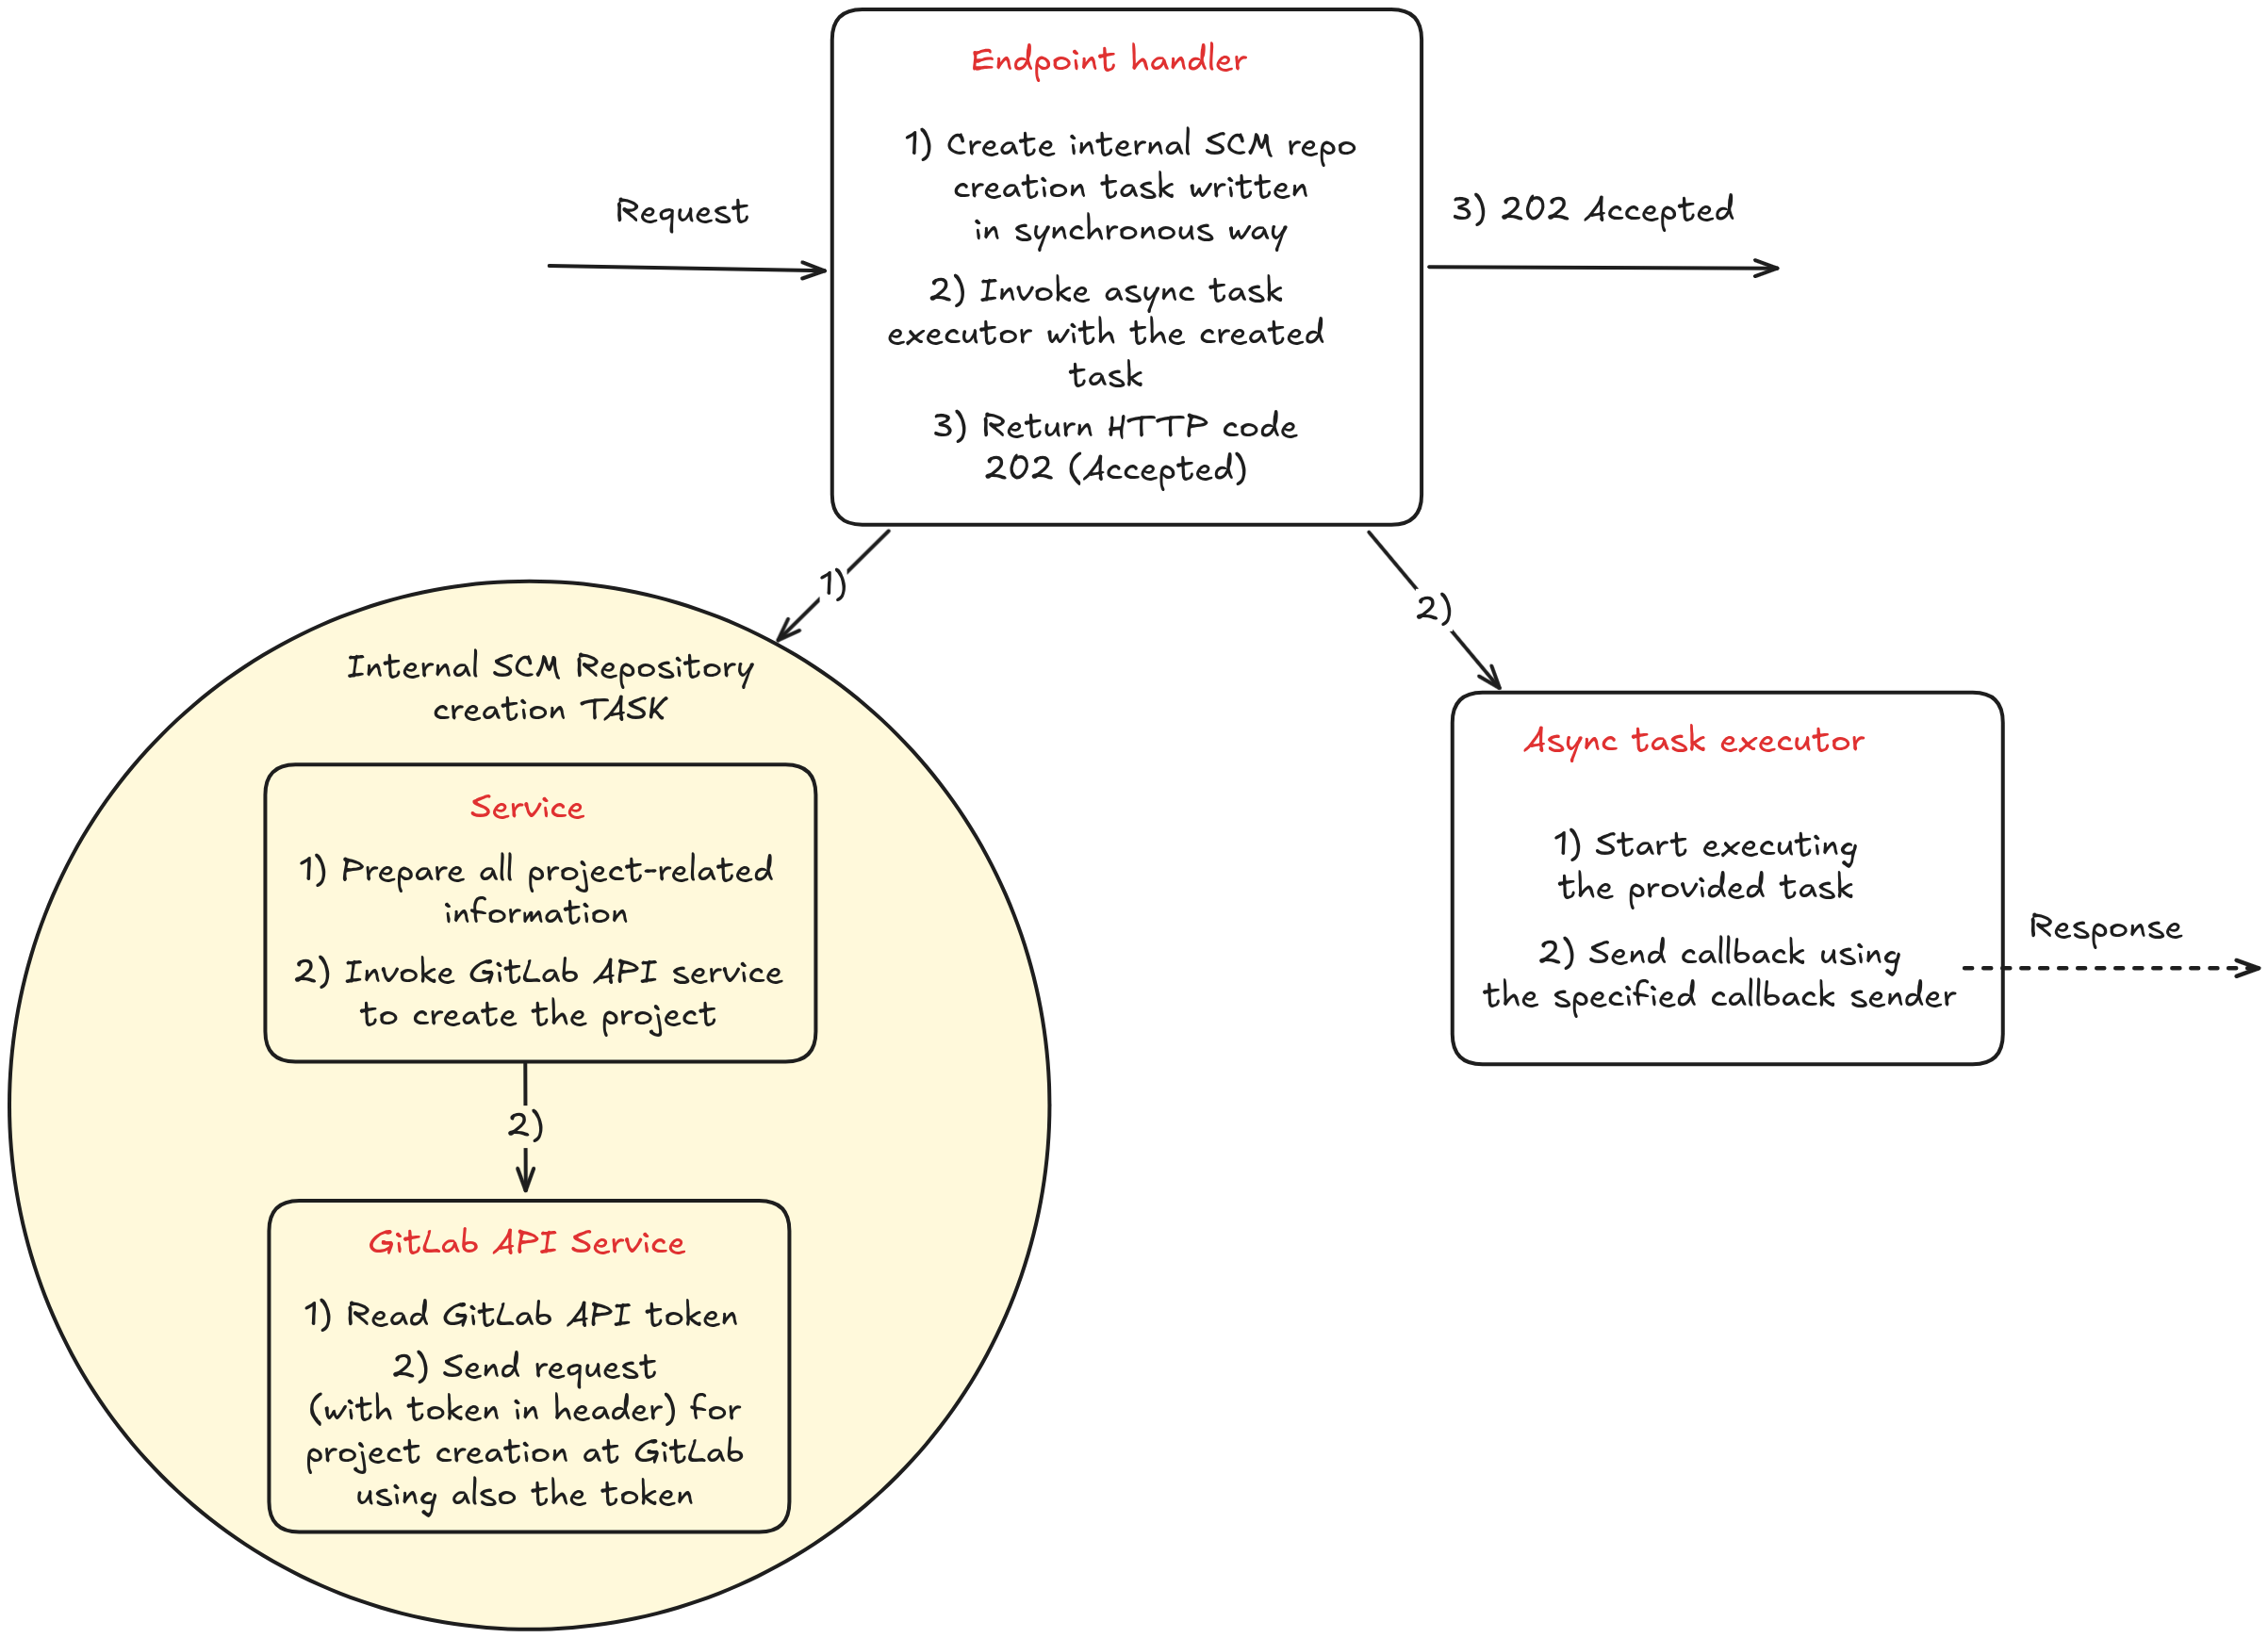
\includegraphics[width=\textwidth]{images/internal-scm-design.png}
  \end{center}
  \caption{Design of internal SCM repository creation}
  \label{fig:internal-scm-design}
\end{figure}

\end{document}
